\section{Analysis of Perceived Randomness}\label{section:analysis_of_perceived_randomness}
As mentioned in Subsection~\ref{subsection:data_analysis}, the analysis of this study's findings is performed using two methods: chi-square goodness-of-fit, and by comparing the differences in cumulative loss of the Learner $L$ and each Expert $\mathcal{E}_i \in \{\mathcal{E}_1,\ldots, \mathcal{E}_N\}$. With these methods, this Chapter delves into the results to provide evidence for the hypothesised question ``are humans good randomisers?'' 

\subsection{Chi-Square Goodness-of-Fit}\label{subsection:chi-square_goodness-of-fit}
We begin with the Chi-Squared ($\chi^2$) Goodness-of-Fit which is a statistical method for determining if the observed results are in line with what is expected from the null hypothesis\textemdash{}that humans are good randomisers.

\subsubsection{Distribution of the Number of Heads}
Figure~\ref{distribution_of_the_number_of_heads} shows that the distribution produced by the subjects is qualitatively similar to the theoretical distribution in that it is bell-shaped, however the results of $\chi^2(10, N=175) = 155.14, p=3.26\mathrm{e}{-28} < 0.0001$ strongly indicate that the binomial distribution is not a good fit, with large discrepancies found at either extreme, and for sequences with $7+$ heads. As noted in~\cite{nickerson:2009}, ``in a randomly produced set of toss sequences, about 25\% of the sequences should have five heads and about 65\% should have four to six heads.'' In this study's sequences, 34\% had exactly five, and 73\% had four to six heads.

\begin{figure}[h]
    \centering
    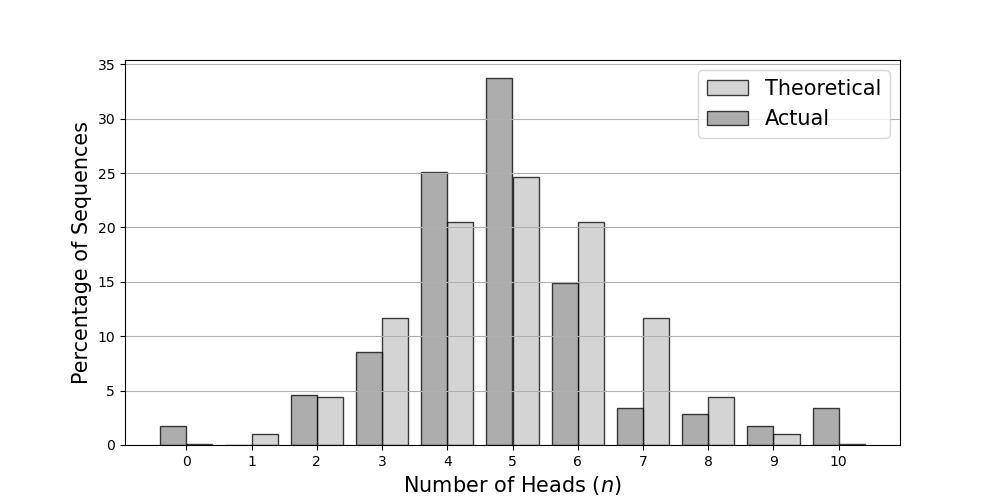
\includegraphics[width=0.9\textwidth]{images/combined_number_of_heads.jpg}
    \caption{Percentage of 10-Item Sequences with $n$ Heads, Compared to the Theoretical Distribution, $X \sim B(10, 0.5)$}
    \label{distribution_of_the_number_of_heads}
\end{figure}

\noindent Overall, these findings are more than significant enough to reject the null hypothesis and support the conclusion noted by Nickerson and Butler in that ``when trying to emulate a random generator of binary sequences, people are likely to produce a larger percentage of sequences that contain the two elements (e.g., heads and tails) in approximately equal proportions than is a random process.''~\cite{nickerson:2009}

\subsubsection{Distribution of the Number of Runs}
Unlike with the Distribution of the Number of Heads, the distribution produced by the subjects shown in Figure~\ref{distribution_of_the_number_of_runs} is both qualitatively and quantitatively different to what was expected, $\chi^2(9, N=175) = 685.64, p=9.29\mathrm{e}{-190} < 0.0001$. The produced distribution does not have a discernable bell-shape, and instead, seems to steadily rise to $r = 8$ before significantly dropping off. 


\begin{figure}[h]
    \centering
    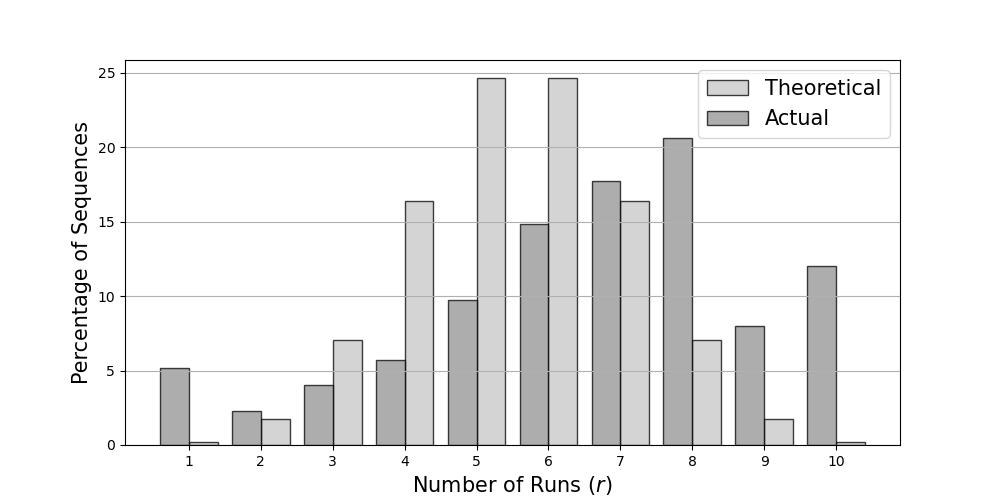
\includegraphics[width=0.9\textwidth]{images/combined_number_of_runs.jpg}
    \caption{Percentage of 10-Item Sequences with $r$ Runs, Compared to the Theoretical Distribution}
    \label{distribution_of_the_number_of_runs}
\end{figure}

Despite looking different to that produced by Nickerson and Butler, this data still supports their conclusion that ``people are likely to fail when trying to emulate a random process-in this case by being less likely than a random process to produce sequences with an intermediate number of runs and more likely to produce sequences with close to the minimum or maximum number possible''~\cite{nickerson:2009}. The discrepancies that follow the peak at $r = 8$ also support Bar-Hillel and Wagenaar's conclusion that ``humans produce series with higher than expected alternation rates''~\cite{bar-hillel:1991}.

\subsubsection{Distribution of Run Lengths}
As previously defined, a \textit{run} is a consecutive sequence of the same outcome (either all heads or all tails), meaning that a run length of 1 occurs when only a single head or tail appears before the outcome changes. While the distribution produced by subjects appears qualitatively similar to the theoretical distribution in that the frequency of run lengths decreases exponentially, a significant percentage of runs more than expected had a length of 1, while all other run lengths were underrepresented in the data, $\chi^2(9, N=1,160) = 33.25, p=0.0001$.

\begin{figure}[h]
    \centering
    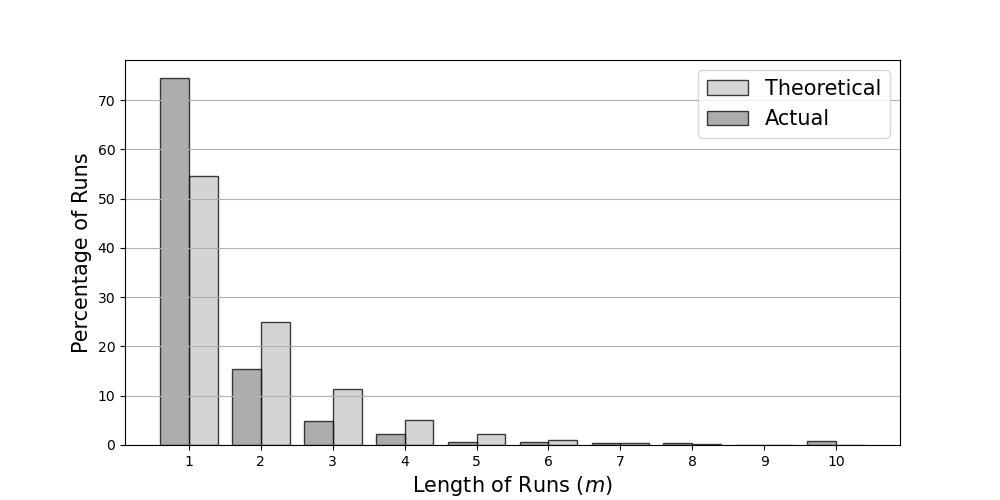
\includegraphics[width=0.9\textwidth]{images/combined_length_of_runs.jpg}
    \caption{Percentage of Runs with Length $m$, Compared to the Theoretical Distribution}
\end{figure}

\noindent Once again, this supports the conclusion drawn by~\cite{bar-hillel:1991} in that human-generated sequences favour alternation over continuation with 90\% of runs across all sequences being up to length $2$, and 97\% being up to length $4$.


\subsection{Regret Analysis}
Given the evidence shown in Subsection~\ref{subsection:chi-square_goodness-of-fit} supporting the conclusion that humans are not good randomisers, we now delve into an evaluation of the Aggregating Algorithm's performance at being able to predict the next bit of human-generated binary sequence.

As previously discussed, a Learner makes use of the predictions from several Experts to form its own about the next bit in a sequence entered by subjects after the fact (acting as Nature in this context). Continuing to assume the null hypothesis that humans are good randomisers, the Aggregating Algorithm should perform no better than randomly guessing the next bit of a sequence, i.e., having a 50\% success rate, however, the plot below shows that this is not the case for any of the subjects tested.

\begin{figure}[h]
    \centering
    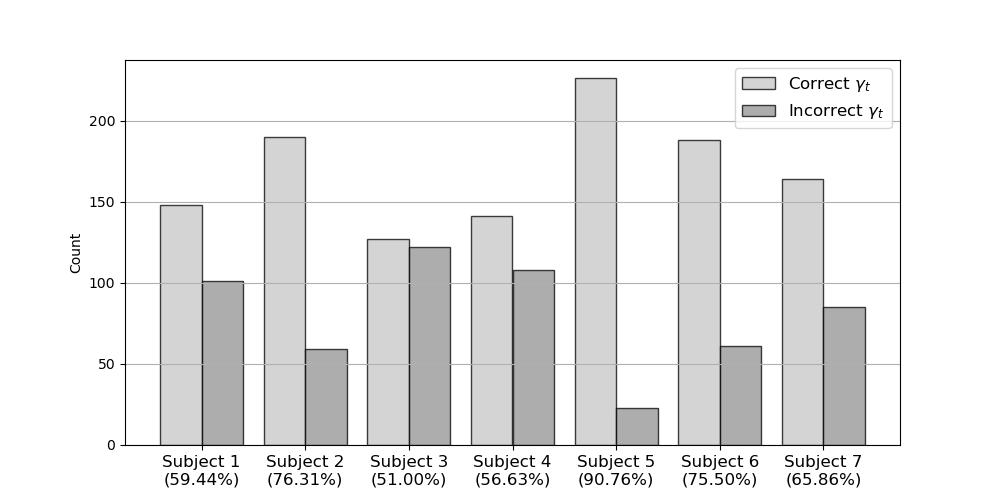
\includegraphics[width=0.9\textwidth]{images/prediction_results.jpg}
    \caption{Correct vs. Incorrect Predictions for Each Subject}
    \label{prediction_results}
\end{figure}

In all cases, the Aggregating Algorithm performed better than random guessing, albeit only marginally for Subject 3. Across the sample, the Aggregating Algorithm had an average accuracy of 67.93\%, further providing evidence that human-generated sequences suffer from predictable patterns, even when considering prefixes up to length $4$.

\begin{itemize}
    \item The closer to objective randomness, the less the difference between each expert and the learner (AH, HA, ME).
    \item The further to obejective randomness, i.e., more predictable, the greater the difference between the expert and the learner (NJ).
\end{itemize}



% \begin{figure}[ht]
%     \centering
%     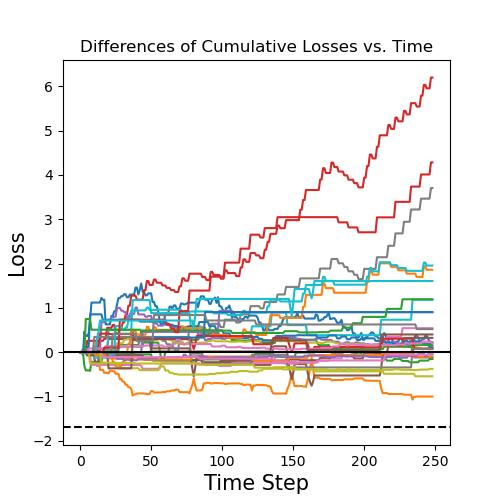
\includegraphics[width=0.625\textwidth]{images/AH_differences.jpg}
%     \caption{Cumulative Loss Differences: Experts vs. Learner for Subject 1}
% \end{figure}
% \begin{figure}[h!]
%     \centering
%     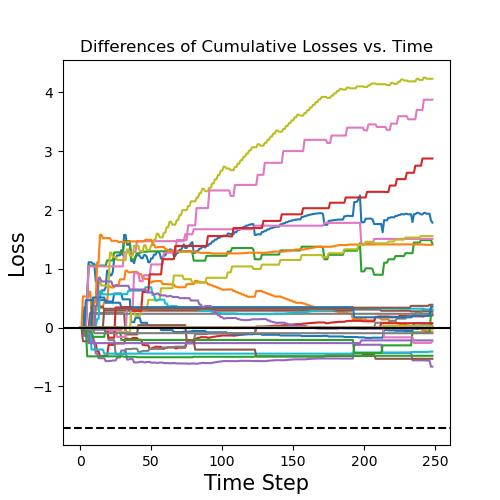
\includegraphics[width=0.625\textwidth]{images/EE_differences.jpg}
%     \caption{Cumulative Loss Differences: Experts vs. Learner for Subject 2}
% \end{figure}
% \begin{figure}[ht]
%     \centering
%     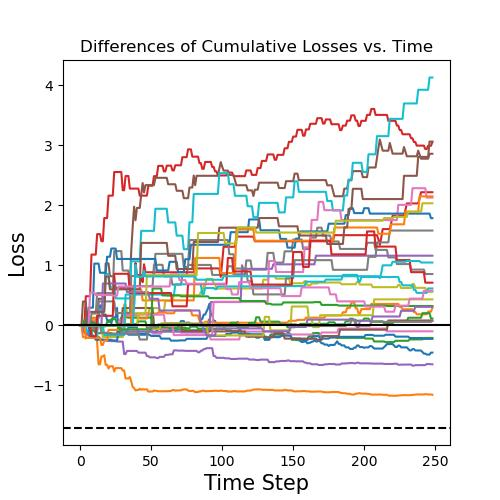
\includegraphics[width=0.625\textwidth]{images/HA_differences.jpg}
%     \caption{Cumulative Loss Differences: Experts vs. Learner for Subject 3}
% \end{figure}
% \begin{figure}[h!]
%     \centering
%     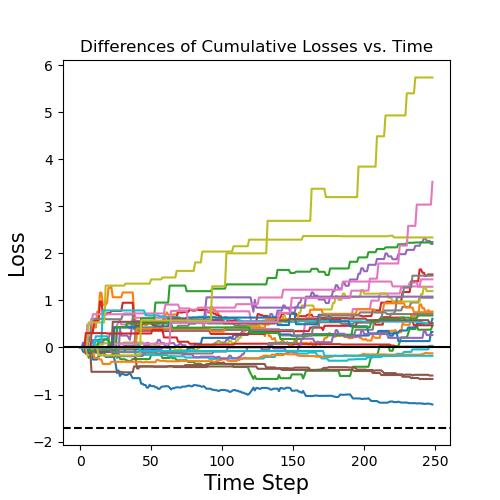
\includegraphics[width=0.625\textwidth]{images/ME_differences.jpg}
%     \caption{Cumulative Loss Differences: Experts vs. Learner for Subject 4}
% \end{figure}
% \begin{figure}[ht]
%     \centering
%     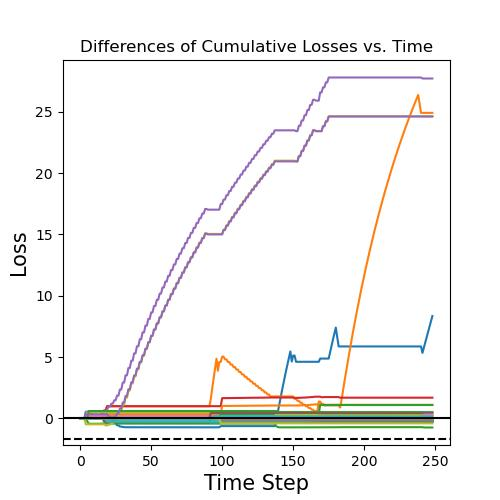
\includegraphics[width=0.625\textwidth]{images/NJ_differences.jpg}
%     \caption{Cumulative Loss Differences: Experts vs. Learner for Subject 5}
% \end{figure}
% \begin{figure}[h!]
%     \centering
%     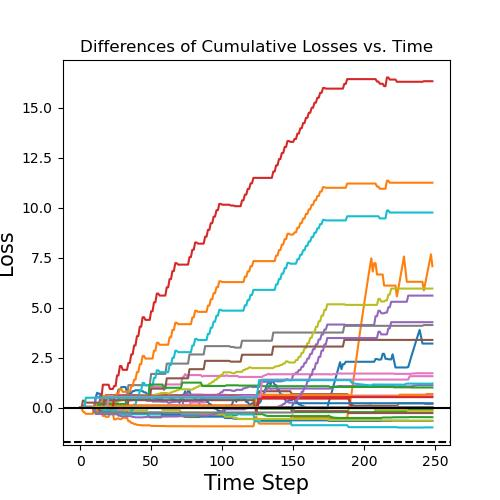
\includegraphics[width=0.625\textwidth]{images/RM_differences.jpg}
%     \caption{Cumulative Loss Differences: Experts vs. Learner for Subject 6}
% \end{figure}
% \begin{figure}[ht]
%     \centering
%     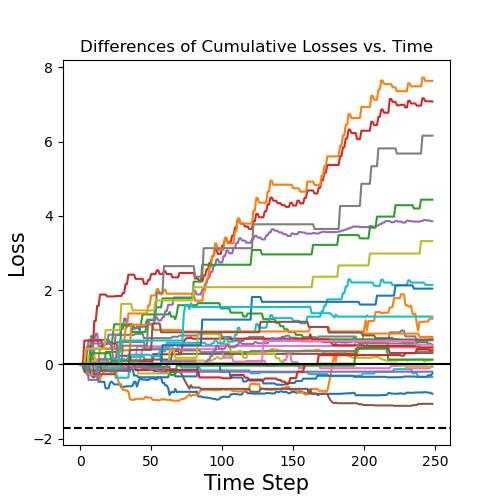
\includegraphics[width=0.625\textwidth]{images/RY_differences.jpg}
%     \caption{Cumulative Loss Differences: Experts vs. Learner for Subject 7}
% \end{figure}


As previously discussed, the Learner uses the predictions of various Experts in order to form its own prediction of the next bit that will be entered by the subject (acting as Nature in this context). The subject's task is to input bits in a way that is random, and thereby unpredictable to the Learner.

In the line chart, when the line is above the x-axis, it means that the difference between the individual expert's loss and the learner's is positive. This means that the expert is performing worse than the learner's method of aggregating predictions.

When the difference is negative, it indicates that the learner is performing worse than the expert, implying that the expert's predictions were close to the actual bits entered by the subject.

If a plot frequently shows the learner's loss being less than that of the experts, it suggests the learner is effectively combining the experts' predicitons and could imply that the subject's bit sequence has some underlying patterns or predictability that the learner is able to exploit, despite the subject's attempt to be random.

Conversely, if the line is frequently above the x-axis, it could indicate that the learner is not effectively aggregating the experts' predicitons, possibly because the subject's sequence is truly random and highly unpredictable. This could suggest that the subject's notion of randomness is strong, and that the learner struggles to predict the next bit accurately.

If the subject's input is truly random, no expert nor the learner should consistently outperform random guessing. The plot might show a mix of positive and negative values, with no clear trend. This randomness would make it difficult for the learner to maintain a consistent advantage.

If the subject's input is only perceived as random, then the learner might perform better over time by effectively leveraging the experts. A plot with the learner frequently outperforming the experts suggests that the subject's sequence is not truly random and that the learner is able to exploit subtle patterns.